\documentclass[12pt]{article}

\usepackage[utf8]{inputenc}
\usepackage[spanish]{babel}
\usepackage{enumerate}
\usepackage{amsmath}
\usepackage{txfonts}
\usepackage{graphicx}
\usepackage{keystroke}
\usepackage{color}
\usepackage[colorlinks = true,
linkcolor = green,
urlcolor = blue,
citecolor = yellow,
anchorcolor = brown]{hyperref}
\usepackage{listings}
\usepackage{alltt}
\usepackage{multicol}

\definecolor{mygreen}{rgb}{0,0.6,0}
\definecolor{mygray}{rgb}{0.5,0.5,0.5}
\definecolor{mymauve}{rgb}{0.58,0,0.82}

\lstset{ %
  backgroundcolor=\color{white},   % choose the background color; you must add \usepackage{color} or \usepackage{xcolor}
  basicstyle=\footnotesize,        % the size of the fonts that are used for the code
  breakatwhitespace=false,         % sets if automatic breaks should only happen at whitespace
  breaklines=true,                 % sets automatic line breaking
  captionpos=b,                    % sets the caption-position to bottom
  commentstyle=\color{mygreen},    % comment style
  deletekeywords={...},            % if you want to delete keywords from the given language
  escapeinside={\%*}{*)},          % if you want to add LaTeX within your code
  extendedchars=true,              % lets you use non-ASCII characters; for 8-bits encodings only, does not work with UTF-8
  frame=single,                    % adds a frame around the code
  keepspaces=true,                 % keeps spaces in text, useful for keeping indentation of code (possibly needs columns=flexible)
  keywordstyle=\color{blue},       % keyword style
  language=Octave,                 % the language of the code
  morekeywords={*,...},            % if you want to add more keywords to the set
  numbers=left,                    % where to put the line-numbers; possible values are (none, left, right)
  numbersep=5pt,                   % how far the line-numbers are from the code
  numberstyle=\tiny\color{mygray}, % the style that is used for the line-numbers
  rulecolor=\color{black},         % if not set, the frame-color may be changed on line-breaks within not-black text (e.g. comments (green here))
  showspaces=false,                % show spaces everywhere adding particular underscores; it overrides 'showstringspaces'
  showstringspaces=false,          % underline spaces within strings only
  showtabs=false,                  % show tabs within strings adding particular underscores
  stepnumber=2,                    % the step between two line-numbers. If it's 1, each line will be numbered
  stringstyle=\color{mymauve},     % string literal style
  tabsize=2,                       % sets default tabsize to 2 spaces
  title=\lstname                   % show the filename of files included with \lstinputlisting; also try caption instead of title
}

\newcommand{\noterm}[1]{\color{blue} \langle #1 \rangle \color{blue}}
\newcommand{\produce}{\color{red} \coloneqq \color{red}}
\newcommand{\alter}{\color{red} \mid \color{red}}
\newcommand{\catterm}[1]{\color{magenta} \text{#1} \color{magenta}}
\newcommand{\term}[1]{\color{cyan} \text{#1} \color{cyan}}
\newcommand{\openopt}{\color{black} \text{[} \color{black}}
\newcommand{\closeopt}{\color{black} \text{]} \color{black}}
\newcommand{\severals}{\color{black} \ldots \color{black}}

\newcounter{ejercicio}
\newcommand{\ejercicio}{\stepcounter{ejercicio}%
  \paragraph\noindent\textbf{Ejercicio \theejercicio.\hspace{4pt}}}

\newcounter{problema}
\newcommand{\problema}{\stepcounter{problema}%
  \paragraph\noindent\textbf{Problema \theproblema.\hspace{4pt}}}
\newcommand{\WindowsLogo}{\raisebox{-0.1em}{%
    \includegraphics[height=0.8em]{../../imagenes/Windows_3_logo_simplified}}}
\newcommand{\WinKey}{\keystroke{\WindowsLogo}}

\newcommand{\Subversion}{\href{https://subversion.apache.org/}{subversion}}
\newcommand{\Riouxsvn}{\href{https://riouxsvn.com/}{Riouxsvn}}

\title{Programación orientada a Objetos en Scala}
\date{2 de marzo de 2021}
\author{S4N Campus}
%\institute{S4N}

\begin{document}
\maketitle

\section{Preliminares}
\label{sec:preliminares}

Este taller tiene como objetivo poner en practica los conceptos vistos en clase sobre el tema de Clases en Scala.

\section{Literales objetos}

\ejercicio Defina un objeto llamado \texttt{comp} con un método
llamado \texttt{cuadrado} que acepte un valor de tipo flotante
(\texttt{Float}) y otro método \texttt{cubo} que acepte un valor de
tipo doble y utilizando el método \texttt{cuadrado} compute el cubo
del valor entrado. $\square$

\ejercicio Pegue y copie el anterior objeto y lo renombra
\texttt{comp2}, pero se debe cambiar todos los tipos para que utilicen
valores de tipo \texttt{Long}. $\square$

\ejercicio Escriba el siguiente código y utilizando el \texttt{REPL} pruebe la salida del siguiente programa, mostrando
el orden de ejecución de las instrucciones.

\begin{lstlisting}[language=Scala]
object prueba {
  def x = {
    println("x")
    1
  }
  val y = {
    println("y")
    x + 2
  }
  def z = {
    println("z")
    x 
    x + "c"
  } 
}
\end{lstlisting}

Una vez cargado el objeto en el \texttt{REPL} ejecute la siguiente instrucción.

\begin{alltt}
scala> prueba.x + prueba.y + prueba.z
\end{alltt}

$\square$

\section{Objetos y clases}
\label{sec:objetos-y-clases}

\ejercicio Dada la siguiente tabla definir la clase \texttt{Gato} y crear un objeto de cada gato de la siguiente tabla.

\begin{center}
\begin{tabular}[h]{|c|c|c|}\hline
  \textbf{Nombre} & \textbf{Color} & \texttt{Comida} \\\hline
  IO & Fawn & Churrus \\
  Make & Red & Leche \\
  Docker & Blue & Cuido \\\hline
\end{tabular}
\end{center}
$\square$

\ejercicio Defina un objeto VentaDeChurrus con un método despachar. Este método debe aceptar un gato y retornar \texttt{true} (Verdadero) si la comida favorita del gato son los Churrus y falso de otra forma. $\square$

\ejercicio Implementar las siguiente clases que se observan en la figura~\ref{fig:escuderia-conductor}

\begin{figure}[h]
  \centering
  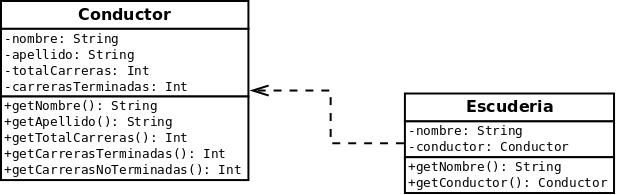
\includegraphics[width=9cm,height=6cm]{imagenes/EscuderiaConductor}
  \caption{Relación de clases Escudería Conductor}
  \label{fig:escuderia-conductor}
\end{figure}

$\square$

\ejercicio Implementar la clase \texttt{Contador} que se observa en la figura~\ref{fig:contador}. El constructor de la clase
debe tomar un entero. Los métodos \texttt{incr} y \texttt{decr} deben retonar ambos un nuevo contador \texttt{Counter}.

\begin{figure}[h]
  \centering
  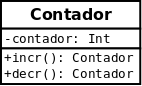
\includegraphics[width=5cm,height=5cm]{imagenes/Contador}
  \caption{Clase contador}
  \label{fig:contador}
\end{figure}

Aquí un ejemplo de uso:

\begin{alltt}
scala > new Contador(10).incr.decr.incr.incr.contador
\end{alltt}

$\square$

\ejercicio Aumentar la clase \texttt{Contador} del anterior ejercicio
que permitas al usuario opcionalmente pasar un parámetro un
\texttt{Int} cómo parámetro da \texttt{incr} y \texttt{decr}. Si el
parámetro es definido este debe ser un valor por omisión de $1$. $\square$


\ejercicio La siguiente código:

\begin{lstlisting}[language=Scala]
class Sumador(monto: Int) {
  def adicionar(valor: Int) = valor + monto
}
\end{lstlisting}

Aumente la clase \texttt{Contador} para adicionar un método que sea
llame \texttt{ajuste}. Este método debe aceptar un \texttt{Sumador} y
retornar un nuevo contador \texttt{Contador} con el resultado de
aplicar el \texttt{Sumador} a el conteo.


\section{Objetos de compañía}
\label{sec:objetos-de-compania}

\ejercicio El siguiente es el código de la clase \texttt{Persona}

\begin{lstlisting}[language=Scala]
class Persona(val nombre: String, val apellido: String) {
  def nombre = s"$nombre $apellido"
}
\end{lstlisting}

Implemente un objeto de compañia para la clase \texttt{Persona} que contenga una método \texttt{apply} que acepte todo el nombre como una sola cadena en vez de un nombre separado por espacios.

\textbf{Pista:} Se puede dividir una cadena dentro de un arreglo de la siguiente forma:

\begin{alltt}
scala> val partes = "Juan Cardona".split(" ")
partes:res0: Array[String] = Array(Juan, Cardona)
scala> partes(0)
partes(0):res1: String = Juan
\end{alltt}

$\square$

\ejercicio La siguientes son las definiciones de dos clases: \texttt{Director} y \texttt{Película}.

\begin{lstlisting}[language=Scala]
class Director (
   val nombre: String,
   val apellido: String,
   val nacimiento: Int) { 
  def nombre: String = s"$nombre $apellido"
  def copy(nombre: String  = this.nombre
           apellido: String = this.apellido,
           nacimiento: Int = nacimiento):Director = 
      new Director(nombre, apellido, nacimiento)
}

class Pelicula (
   val nombre: String
   val presentacion: Int,
   val rangoIMDB: Double
   val director: Director) {

  def directorEdad = presentacion - director.nacimiento
  def esDirigidaPor(director:Director) = 
      this.director == director
  def copy(
      nombre:String = this.nombre,
      presentacion = this.presentacion,
      rangoIMDB:Double = this.rangoIMDB,
      director:Director = this.director):Pelicula = 
      new Pelicula(nombre,presentacion,rangoIMDB,director)
}
\end{lstlisting}

Escriba objetos de compañía para las clases \texttt{Director} y \texttt{Pelicula} como sigue:

Para \texttt{Director}:

\begin{itemize}
\item Un método \texttt{apply} que acepte los mismos parámetros del constructor de la clase y retorne un
  nuevo \texttt{Director}.
\item Un método \texttt{esMayor} que acepte dos \texttt{Director}(es) y retorne el mayor de los dos.
\end{itemize}

Para \texttt{Pelicula}:

\begin{itemize}
\item Un método \texttt{apply} que acepte los mismos parámetros del constructor de la clase y retorne un
  nuevo \texttt{Pelicula}.
\item Un método \texttt{mejorCalificada} que acepte dos
  \texttt{Pelicula}(s) y retorna la que tiene mayor \texttt{rangoIMDB}
  entre las dos.
\item Un método \texttt{mayorDirectorEnElTiempo} que acepte dos \texttt{Pelicula}(s) y retorne el \texttt{Director} que fue mayor
  en el momento de presentar la película.
\end{itemize}

$\square$

% \section{Bibliografía}
% \label{sec:bibliografia}
% \bibliographystyle{amsalpha}
% \bibliography{S4N_Git_Tutorial}

\end{document}

%%% Local Variables:
%%% mode: latex
%%% TeX-master: t
%%% End:
